\chapter{Các thuật toán Unsupervised Learning}

% ==========================================
% SECTION 1: K-MEANS CLUSTERING
% ==========================================
\section{K-Means Clustering}

\begin{figure}[H]
    \centering
    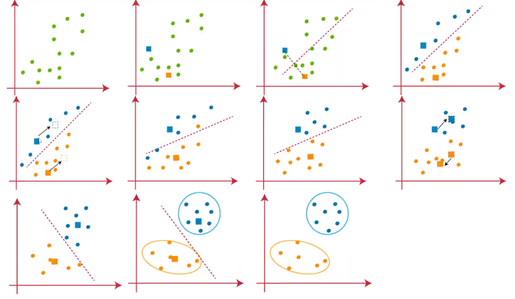
\includegraphics[width=0.8\linewidth]{41.png}
    %\fbox{\parbox[c][4cm][c]{0.8\linewidth}{\centering \textit{[Chèn ảnh: Minh họa thuật toán K-Means Clustering tại đây]}}}
    \caption{Nguyên lý phân cụm của thuật toán K-Means Clustering}
    \label{fig:kmeans}
\end{figure}

\begin{itemize}
    \item Liên tục lặp lại hành động chọn tâm cụm (center/centroid) và cập nhật lại vị trí tâm dựa trên giá trị trung bình của các điểm dữ liệu thuộc nhóm đã phân chia trước đó.
    \item Quá trình này được lặp đi lặp lại cho đến khi hội tụ — tức là khi vị trí của các tâm cụm không còn thay đổi nữa.
\end{itemize}